\documentclass{article}

\usepackage[dutch]{babel}
\usepackage{epsfig}
\usepackage{verbatim}
\usepackage{amsmath}

\author{Peter van Dijk \& Elizabeth Schermerhorn}
\date{\today}
\title{Localisatie met Arduino\'s op basis van vier bakens}
\begin{document}
\maketitle
\newpage
\tableofcontents
\clearpage
\section{Inleiding}
In deze paper zal een localisatie algoritme besproken worden. De localisatie zal gedaan worden op basis van vier bakens die een ultrasoon geluid uitzenden en een arduino met een ultrasoon ontvanger. Het doel van dit experiment is om binnen een 5m bij 5m veld de positie zo nauwkeurig mogelijk proberen te bepalen. Aan de hand van het ultrasone geluid in combinatie met een GPS-bepalings algoritme wordt nauwkeurig bepaald wat de co\"{o}rdinaten zijn. 


\section{Probleemstelling}
De onderzoeksvraag die hier centraal staat: \textit{"Een algoritme opstellen waarmee de exacte GPS-positie te bepalen is."} 
De hypothese is dat dit  gaat lukken. Aangezien het om een statische omgeving gaat waarbinnen alles te controleren is zou dit mogelijk moeten zijn. Door het signaal van de bakens te ontvangen kan de afstand tot de individuele bakens berekend worden. Vervolgens kan met een GPS-algoritme de precieze locatie bepaald worden. Een verwacht obstakel hierbij zal de overflow(Getallen zijn te groot om te representeren) in arduino zijn. 

\section{Gerelateerd werk}
Op dit gebied is er al veel onderzoek verricht. Hierdoor is er veel werk wat gebruikt kan worden bij het onderzoek. Aangezien dit een onderzoek is wat al vele malen is uitgevoerd is er veel gerelateerd werk wat is gebruikt in dit onderzoek. In deze twee papers worden er globale localisatie systemen beschreven en hoe deze gebruik maken van externe factoren. In de volgende twee papers worden er GPS-bepalings algoritmen gepresenteerd waarmee de exacte locatie bepaald kan worden. In de eerste twee papers worden twee manieren toegelicht waarop localisering mogelijk is. In [http://www.cl.cam.ac.uk/research/dtg/www/publications/public/files/tr.97.10.pdf] worden twee manieren beschreven, namelijk:
\begin{itemize}
	\item Active badges
	\item ParcTab
\end{itemize}

Active badges is gebasseerd op het periodiek verzenden van informatie naar iedereen. Door -bijvoorbeeld een gebouw - heen zijn er overal sensoren geplaatst die luisteren naar berichten die worden verstuurd door badges. Door vast te stellen welke sensoren het signaal van welke badge hebben ontvangen is het mogelijk een grove schatting te g
even van de locatie van de badge.
\newline 

ParcTab is een PDA die gebruik maakt van infrarood voor het netwerk.Wat betreft de localisatie bepaling lijkt deze heel veel op de badges die hierboven staan beschreven. Er worden berichten verstuurd en afhankelijk van welke sensor deze ontvangen wordt de locatie bepaald. Een groot verschil is dat de ParcTab is bedoeld voor veel meer en intensiever gebruik dan alleen de localatie berekenen. 

In de laatste twee papers, [http://en.wikipedia.org/wiki/Trilateration] en [Localization and positioning, CH. 9] worden er twee manieren besproken waarop de GPS positie bepaald kan worden. 

In hoofdstuk 9 van Localization and positioning wordt er ook gebruik gemaakt van bakens die een signaal uitzenden. Er moet eerst berekend worden wat de afstand is tot de verschillende bakens. Voor dit algoritme is het van belang dat er minimaal tot drie bakens de locatie bekend is. Wanneer de afstand tot drie bakens bekend is wordt er gebruik gemaakt van matrixberekeningen om de locatie te bepalen. Dit is de implementatie die ook is gebruikt in het experiment wat in deze paper is gemaakt.
\newline
Een tweede GPS-positie bepaling die gebruikt zou kunnen worden heet triangulation. Ook hier wordt gebruik gemaakt van de afstand tot de bakens die een signaal verzenden. Dit algoritme lijkt veel op het algoritme uit CH9 maar hier wordt gebruik gemaakt van de berekening van cirkels waardoor er geen matrixberekeningen nodig zijn. 




\section{Instellingen}
Om deze hypothesen te toetsen moeten er metingen gedaan worden. Hier zijn verschillende zaken van belang. 
\begin{itemize}
	\item De gebruikte hardware
	\item De gebruikte software
	\item De instellingen/vastgestelde constanten
	\item De onderzoeksopstelling
\end{itemize}

%De gebruikte hardware
\subsubsection{De hardware}
De Hardware die gebruikt is bij de metingen is een Arduino UNO en een Nordic nRF24L01 draadloze transceiver in combinatie met een ultrasoonontvanger. \\

%de gebruikte software
\subsubsection{De software}
Om de hardware te gebruiken wordt gebruik gemaakt van de opensourcesoftwarebibliotheek voor de Arduino, die te vinden is op: \begin{verbatim}http://maniacbug.github.io/RF24/ \end{verbatim} 
Met deze software kunnen de radio en ontvanger aangestuurd worden en kunnen pakketjes worden verzonden en ontvangen. De radio luistert en verstuurt pakketten over een bepaald kanaal. Het is van belang dat de radio's hetzelfde kanaal gebruiken, zodat ze met elkaar kunnen communiceren. De kanalen hebben een nummer van 0 tot en met 125. De radio heeft de volgende instellingen nodig:
\begin{itemize}
	\item Kanaal 76 
	\item Automatisch herverzenden Uit
	\item Transmissiesnelheid: 2 Mbps
	\item Adres verzendende pipe: 0xdeadbeefa1LL
	\item Payload-grootte 1 byte
\end{itemize}
De ultrasoon ontvanger moet op een bepaalde manier aangesloten worden zodat deze geluid kan ontvangen:
\begin{tabular}{l| l}
\hline
afkorting & Wijze van aansluiten \\ \hline
E & Verbinden met GND van Arduino \\
GN & Verbinden met 5V van Arduino \\
++ & Verbinden met 5V van Arduino \\
GND & Verbinden met Ground van Arduino \\
S & niet aansluiten \\
\end{tabular}
\\
\\
Om de tests te kunnen uitvoeren is er gebruik gemaakt van vier bakens die met een bepaald patroon informatie verzenden. In grafiek  XXXXX is schematisch weergegeven hoe de signaal verzending werkt. In het schema zijn vier dezelfde iteraties te zien. Omdat er gebruik wordt gemaakt van vier bakens staan er vier berichten in het schema weergegeven. 
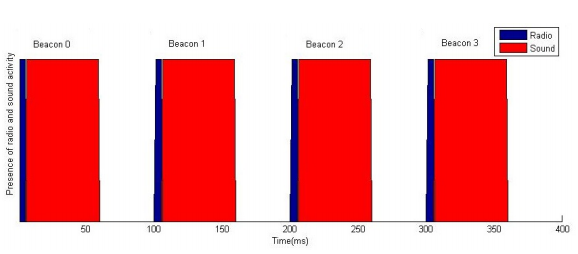
\includegraphics{berichten_bakens}



\section{Het algoritme}
Het algoritme wat ge\"{i}mplementeerd is, bestaat uit twee verschillende onderdelen. Het bestaat uit een deel afstand berekenen tot de verschillende bakens, en de uiteindelijke GPS-bepaling. 
Deze twee onderdelen zullen apart besproken worden voor de overzichtelijkheid.
	
\subsection{Afstand bepalen tot aan de bakens}
	Zoals te zien is in FIGUUR WAAR REF NIET LUKT :( wordt er eerst een radio signaal verstuurd gevolgd door een ultrasoon signaal. Het versturen van een ultrasoon bericht wordt door een master-baken bepaald. Als eerste wordt er door de master-baken een radio bericht uitgezonden naar iedereen met het bericht welke baken mag sturen. Omdat dit een radiosignaal is gaat dit met de snelheid van het licht, dit signaal propageert zo snel voort dat wanneer een node een meter dichterbij staat dit verwaarloosbaar is geworden. Op het moment dat het radio signaal ontvangen wordt, begint de baken direct met een ultrasoon geluid versturen. Doordat bekent is dat dit meteen gebeurt wordt er bijgehouden hoelang het duurt voordat er een bericht wordt ontvangen. Op het moment dat het bericht wordt ontvangen wordt er met behulp van de geluidssnelheid berekend wat de afstand tot de baken is. Het is van belang om een juiste geluidssnelheid te kiezen bij de omgeving waarin het systeem staat, de afwijkingen kunnen groot zijn. Dit proces van luisteren en berekenen herhaalt zich oneindig lang zodat wanneer de node in beweging is er nog steeds een correcte locatie gegeven kan worden. 
	
\subsection{GPS-positie bepaling}
Nu van alle vier de bakens bekend is wat hun afstand is tot de node kan door middel van matrixberekeningen de positie worden bepaald. Hierbij is er gebruik gemaakt van [https://blackboard.utwente.nl/bbcswebdav/pid-724118-dt-content-rid-1165054_2/courses/2013-201200005-2B/Protocols%20and%20Architectures%20for%20wireless%20sensor%20networks-ch9.pdf]. 
Hiervoor was het nodig om de GPS-posities van de bakens te hebben waar de waarden op gebaseerd kunnen worden. 

\section{Resultaten en analyse}

  
\section{Metingen en resultaten}

\section{Conclusie}

\newpage
